% durch Austauschen dieser Zeilen kann die Sprache des Templates geändert werden
\PassOptionsToPackage{main=ngerman}{babel}
%\PassOptionsToPackage{main=english}{babel}

\documentclass{mi-thesis}

\bachelor % im Falle einer Masterarbeit \master

% Variablen, die für das Deckblatt und Metadaten verwendet werden
\title{[Titel der Bachelor-/ Masterarbeit]}
\author{[Autor*in der Arbeit]}
\semester{[WS / SS und Jahreszahl]}
\course{[Art des Seminars und Seminartitel (z.B. Praktikum Multimedia Engineering)]}
\module{[z.B. MEI-M 04 (B.A.)]}
\dozent{[Seminarleiter]}
\studid{[Matrikelnummer]}
\studSemester{[Semesterzahl und Studiengänge (z.B. 3. Semester B.A. Medieninformatik / Informationswissenschaft)]}
\phone{0941/133742666} % Optional
\studSubject{Medieninformatik}
\firstReviewer{Prof. Dr. Maike Musterprof}
\secondReviewer{Prof. Dr. Max Musterprof}
\advisor{Momo Mustermensch}
\address{Domplatz 1, 93047 Regensburg}{} % Optional
\mail{[Emailadresse (z.B.: max.mustermann@stud.uni-regensburg.de)]}
\studMail{[Emailadresse (z.B.: max.mustermann@stud.uni-regensburg.de)]}
\dateHandedIn{[Abgabetermin der Arbeit]}
\keywords{Enter;key;words;here}

\bibliographystyle{apacite}

% Falls Sie die Abkürzung zum Einbinden von Grafiken benutzen möchten. Erläuterung fnden Sie im Abschnitt zu Abbildungen.
\newcommand*{\image}[2]{
	\begin{figure}
	\centering
	\includegraphics[width=0.5\textwidth]{{images/#1}}
	\caption{#2}
	\label{fig:#1}
	\end{figure}
}

\begin{document}

% Die Nummerierung beginnt mit der Titelseite (= Seite 1), soll aber erst ab der ersten Inhaltsseite (Einleitung) angezeigt werden.
\pagestyle{empty}

% Deckblatt des Templates und Hinweise
% diese Zeile für die Verwendung des Templates entfernen!
\begin{titlepage}
\sffamily
\centering

\includegraphics[width=0.5\textwidth]{{images/logo_uni}}

\vspace{5cm}

\huge\bfseries
Richtlinien und Vorlage\\
zur Gestaltung\\
schriftlicher Arbeiten

\vspace{1cm}

\Large\mdseries Lehrstuhl für Medieninformatik

\medskip
Universität Regensburg

\vspace{5mm}

\onehalfspacing
\normalsize
Version 4.4

Februar 2022

\end{titlepage}


\section*{Hinweise zur Verwendung dieser Richtlinien/Vorlage}

\begin{itemize}
    \item Dieses Dokument dient sowohl als Formatvorlage für Seminar- und Abschlussarbeiten, als auch als Sammlung von Richtlinien für diese Arbeiten.
    \item Achten Sie insbesondere auf eine korrekte Seitennummerierung. Die Nummerierung beginnt mit der Titelseite (= Seite 1), soll aber erst ab der ersten Inhaltsseite (Einleitung) angezeigt werden.
    \item Verwendete Schriftarten und Alternativen:
    \begin{itemize}
        \item Fließtext und Überschriften: Palatino Linotype (Windows, unter Mac OS X nur mit Drittsoftware installiert), alternativ Book Antiqua (Mac OS X) oder TeX Gyre Pagella (freie Lizenz).
        \item Sans-serif wenn benötigt: Frutiger Next LTW1G, Helvetica, Nimbus Sans.
        \item Code-Beispiele: beliebige Monospace-Schriftart, z.B. Courier New, Consolas, Droid Sans Mono, DejaVu Sans Mono.
    \end{itemize}
\end{itemize}


\section*{Änderungshistorie}


\begin{tabularx}{\textwidth}{@{}llX@{}}
\toprule
\bfseries Version & \bfseries Datum & \bfseries Änderungen \\
\midrule
4.4 & 2022-02-01 & Einige Änderungen auf Basis von Github-Issues, es kann nun über Package-Parameter zwischen Seminar- und Abschlussarbeit gewechselt werden \\
\midrule
4.3 & 2020-03-31 & Inhalt des \LaTeX-Templates an die anderen Templates angepasst \\
\midrule
4.2 & 2016-10-31 & Aufgabenstellung, Name/Titel bei Rechteerklärung hinzugefügt \\
\midrule
4.1 & 2016-06-01 & Umfangreiche Anpassung Plagiatserklärung, Abb.-, Tabellen- und Stichwortverzeichnis sind explizit als optional gekennzeichnet. Beispiele für die Zusammenfassung hinzugefügt, Reparatur defekter Formatierungen, Seitenzahlen. Logo auf Titelseite BA/MA kleiner.
Neu: Obenstehende Hinweise, Seitenheader. Inhaltsverzeichnis für Datenträger Erklärung zur Lizenz und Publizierung. \\
\bottomrule
\end{tabularx}


% Das Deckblatt erstellen
\maketitle

\tableofcontents % Optional
\listoffigures % Optional
\listoftables % Optional
\lstlistoflistings % Optional


\clearpage
\doublespacing

\begin{abstract}
Bachelor- und Masterarbeiten beginnen mit einer Zusammenfassung in einer deutschen und englischen Version.
Die Zusammenfassung gibt einen Überblick über Thema und Resultate der Arbeit.
Inhaltlich werden die Zielsetzung, die Methodik, die einzelnen Arbeitsschritte bzw. Gliederungspunkte und die Ergebnisse der Arbeit widergegeben.

Schlecht: „Schon immer haben Menschen Zusammenfassungen geschrieben [Platitüde, keine Zusammenfassung]. In dieser Arbeit wurde in mehreren Studien untersucht, wie Zusammenfassungen wirken. [Was genau wurde untersucht? Was waren die Ergebnisse?]“

Besser: „In dieser Arbeit wurde untersucht, inwiefern das Lesen von Zusammenfassungen das Lesen des kompletten Dokuments ersetzen kann. Dazu wurden zwei Studien mit jeweils 17 Teilnehmern durchgeführt. In der ersten wurde [...]. Diese Ergebnisse zeigen, dass Bedienungsanleitungen und Bilderbücher weniger gut über Zusammenfassungen erschlossen werden können, als Romane oder Sachbücher.“
\end{abstract}

\begin{abstract}[english]
A summary in English. It should be more or less similar to the German Zusammenfassung. Avoid too verbatim translations („In this work it was examined how the reading of ...“)
\end{abstract}


\clearpage
\pagestyle{headings} % Seitennummern und Kapitelbezeichnungen anzeigen

% hier beginnt der eigentliche Inhalt der Arbeit

\addchap{Aufgabenstellung}\label{sec:Aufgabenstellung}

Die Aufgabenstellung beschreibt sowohl allgemein als auch konkret, was das Ziel der Arbeit ist, und wie dieses erreicht werden soll. 
In der Regel wird die Aufgabenstellung vom Betreuer der Seminar- oder Abschlussarbeit grob vorgegeben und dann gemeinsam konkretisiert. Bei Abschlussarbeiten ist in der Regel schon eine Aufgabenstellung auf der Wiki-Seite zur Arbeit zu finden. Diese kann je nach Ausführlichkeit direkt übernommen oder als Basis für die hier dokumentierte Aufgabenstellung dienen. 

Die Aufgabenstellung muss vor Anmeldung der Arbeit mit dem Betreuer abgestimmt werden. Bitte beachten Sie auch die Qualitätskriterien für Themen, die im Wiki dokumentiert sind.
Die Aufgabenstellung sollte in der Regel aus drei Abschnitten (ohne eigene Überschriften) bestehen: 

\begin{itemize}
    \item{Hintergrund/Motivation}
    \item{allgemeine Zielsetzung und Herangehensweise}
    \item{konkrete einzelne Schritte zum Erreichen des Ziels}
\end{itemize}

\chapter{Einleitung}\label{sec:Einleitung}

Dieses Dokument soll für die Gestaltung von wissenschaftlichen Arbeiten wie Seminararbeiten, Projektdokumentationen, Bachelorarbeiten oder Masterarbeiten am Lehrstuhl für Medieninformatik dienen. Es kann direkt als Word-Vorlage oder nur als Referenz zur Formatierung mit anderen Textsatzprogrammen verwendet werden. 

Ausgehend von den Zielen der Vorlage, werden empfehlenswerte Lehrbücher zum Thema sozusagen als Stand der Technik vorgestellt. Danach werden im Punkt „Gestaltungsrichtlinien“ die Vorgaben für inhaltliche und formale Gestaltung, sowie Zitierweise erläutert. In einem weiteren Abschnitt finden sich Literaturhinweise für empirische Arbeiten sowie Tipps für die Darstellung der Ergebnisse.

Diese Richtlinien dürfen gerne ganz oder teilweise als Grundlage für eigene Richtlinien anderer Lehrstühle verwendet werden. Als Quellenangabe kann „Richtlinien zur Gestaltung schriftlicher Arbeiten, Lehrstuhl für Medieninformatik der Universität Regensburg, Version X.X“ verwendet werden.

\chapter{Ziele}\label{Ziele}

Die formalen und inhaltlichen Gestaltungsrichtlinien der Dokumentvorlage sollen folgenden Zielen dienen:

\begin{enumerate}
    \item{Die Vorlage soll die Erstellung formal und inhaltlich korrekter Arbeiten mit Word erleichtern.}
    \item{Die formulierten Richtlinien können als Referenz für die Erstellung von wissenschaftlichen Arbeiten mit anderen Textverarbeitungsprogrammen dienen.}
\end{enumerate}

\chapter{Stand der Technik}\label{sec:stand_der_technik}

Es gibt zahlreiche Ratgeber\index{Ratgeber} für das wissenschaftliche Arbeiten und Schreiben. Die Handbücher unterscheiden sich in inhaltlichen Schwerpunkt, praktischer Orientierung und Vertiefung der einzelnen Themen. Drei sehr empfehlenswerte Ratgeber sollen kurz vorgestellt werden.

\cite{karmasin2012gestaltung} bieten einen sehr knappen und praktisch orientierten Ratgeber. Es werden inhaltliche und formale Anforderungen an wissenschaftliche Arbeiten wie inhaltlicher Aufbau der Kapitel, Bewertungskriterien und formale Aspekte wie Gliederung behandelt. Daneben enthält der Ratgeber ein eigenes Kapitel mit Tipps zur Formatierung mit Word.

Das Handbuch von \cite{esselborn2012richtig} konzentriert sich auf die Frage nach dem richtigen wissenschaftlichen Sprachstil. Es werden konkrete Regeln und Übungen vorgestellt um sprachliche Präzision und gedankliche Klarheit im Text zu erreichen. Daneben wird in einem eigenen Kapitel auf die häufigsten Fehler beim wissenschaftlichen Schreiben hingewiesen.

\cite{balzert2011wissenschaftliches} bieten einen sehr ausführlichen Ratgeber zum wissenschaftlichen Arbeiten. Im ersten Teil werden Qualitätskriterien und Methoden als Grundlagen wissenschaftlicher Arbeit aufgezeigt. Im zweiten Teil werden verschiedene wissenschaftliche Artefakte also Textformen gegenübergestellt und der formale Aufbau wissenschaftlicher Arbeiten beleuchtet. Im dritten Teil werden Empfehlungen zum Erstellungsprozess einer Arbeit mit Projektplan etc. gegeben. Im letzten Teil werden verschiedene Aspekte der Präsentation behandelt, wie z. B. Vortragsformen mit und ohne visuelle Unterstützung oder der richtige Vortragsstil.

\chapter{Gestaltungsrichtlinien}\label{sec:gestaltungsrichtlinien}

\section{Sprache\index{Sprache} und Textumfag}\label{subsec:sprache_textumfang}

Laut Prüfungsordnung dürfen Bachelor- und Masterarbeiten in deutscher oder englischer Sprache verfasst werden.
Weitere Sprachen sind nach Absprache mit dem Prüfungsausschuss möglich.
Der geeignete Umfang von wissenschaftlichen Arbeiten ist abhängig von Thema, Schreibstil des Verfassers und Anzahl der Verfasser.
Generell sollte man sich an folgenden Richtwerten orientieren.
Die Werte beziehen sich auf den reinen Text ohne Inhaltsverzeichnis\index{Inhaltsverzeichnis}, Literaturverzeichnis oder Anhänge.

\begin{itemize}
    \item{Seminararbeiten ca. 20-30 Seiten}
    \item{Projektdokumentationen ca. 20-40 Seiten}
    \item{Bachelorarbeiten ca. 30-50 Seiten}
    \item{Masterarbeiten ca. 60-80 Seiten}
\end{itemize}

\section{Inhaltliche Bestandteile}\label{subsec:inhaltliche_bestandteile}

Jede Arbeit besteht aus den folgenden Bestandteilen in der vorgegebenen Reihenfolge.
Dabei beginnt jeder Abschnitt auf einer neuen Seite. 

\begin{enumerate}
    \item{Titelseite}
    \item{Inhaltsverzeichnis}
    \item{Abbildungsverzeichnis (optional)}
    \item{Tabellenverzeichnis (optional)}
    \item{Zusammenfassung/Abstract (bei Seminararbeiten und Projektdokumentationen optional)}
    \item{Einleitung}
    \item{Hauptteil}
    \item{Schluss}
    \item{Literaturverzeichnis}
    \item{Erklärung zur Urheberschaft}
    \item{Anhang (optional)}
    \item{Index (optional)}
\end{enumerate}

\minisec{Titelseite}\index{Titelseite}

Die Titelseite enthält alle wichtigen Angaben zu Lehrveranstaltung (Semester, Universität, Lehrveranstaltung, Dozent, Modul), den Titel der Arbeit (im genauen Wortlaut der Themenstellung), Angaben zum Verfasser (Name, Anschrift, E-Mailadresse, Matrikelnummer, Semesterzahl, Datum der Abgabe).
Zusätzlich werden bei Bachelor- und Masterarbeit Erst-und Zweitgutachter angegeben.

\minisec{Inahltsverzeichnis}

Das Inhaltsverzeichnis enthält alle Gliederungspunkte auf allen Ebenen mit den entsprechenden Seitenzahlen.
Es sollen nicht mehr als drei bis maximal vier Gliederungsebenen (1.1.1.1) verwendet werden. Die Nummerierung erfolgt in Dezimalgliederung (1., 1.1 usw.).
Inhaltsverzeichnis und Plagiatserklärung\index{Plagiatserklärung} werden im Inhaltsverzeichnis aufgeführt, aber nicht nummeriert.

\minisec{Einleitung}\index{Einleitung}

Die Einleitung muss nicht zwingend kreativ oder originell sein, sondern ergibt sich aus der Arbeit.
Da sich der genaue Inhalt und die Ergebnisse während der Bearbeitung ändern können, muss die Einleitung eventuell später angepasst werden.
Inhaltlich grenzt die Einleitung das Thema genau ein mit Formulierungen wie „diese Arbeit beschäftigt sich mit XY“.
Danach sollte aufgezeigt werden, inwiefern die Problemstellung für die Medieninformatik relevant ist, sowie die einzelnen Ziele der Arbeit.
Abschließend wird der inhaltliche Aufbau der Arbeit erläutert.
Allgemeinplätze wie „immer mehr Menschen verwenden Computer“ sollten unbedingt vermieden werden.

\minisec{Hauptteil}\index{Hauptteil}

Der Hauptteil beginnt mit einem kurzen Kapitel zu den Zielen der Arbeit.
Bei sehr kurzen Arbeiten, wie einer Seminararbeit, ist dieser Punkt meist mit der Einleitung schon abgedeckt.
Darauf folgt der aktuelle Forschungsstand zum Thema.
Dabei werden unterschiedliche Ansätze vorgestellt und ihre Vor- und Nachteile aufgezeigt.
Je nach Art des Themas fallen die weiteren inhaltlichen Bestandteile unterschiedlich aus.
Im Anhang\index{Anhang} A befinden sich die inhaltlichen Bausteine für eine theoretische, eine konstruktive (Paradigma der „Design Science“) oder eine empirische Arbeit (Paradigma der „Behavioral Science“).

\minisec{Schluss}\index{Schluss}

Im Schlussteil soll deutlich werden, was innerhalb der Arbeit erreicht wurde.
Dazu kann man sich auf die Anfangs beschriebenen Ziele oder Hypothesen beziehen und die wichtigsten Schritte und Erkenntnisse zusammenfassen.
Nach den Ergebnissen kann zusätzlich ein Ausblick gegeben werden, wie sich das Problem weiterentwickeln wird, oder welche weiteren Forschungsfragen sich an die Arbeit anknüpfen.

\minisec{Erklärung zur Urheberschaft}

Eine unterschriebene \emph{Erklärung zur Urheberschaft} ist der Bachelor- und der Masterarbeit beizulegen. Bei der Abgabe von digitalen Arbeiten, z.B. Hochladen einer PDF-Datei auf Grips, reicht die Erklärung ohne Unterschrift aus.
Den konkreten Text der Erklärung finden Sie in der nach dem Anhang.

\minisec{Index}\index{Index}

Bei umfangreichen Arbeiten kann ein Sachwortverzeichnis oder Index sinnvoll sein.
Der Index enthält am Ende der Arbeit bedeutende Schlagworte und dazugehörige Seitenangaben.

\minisec{Anhang}

Material, das innerhalb der Arbeit benutzt wurde oder entstanden ist wie Fragebögen, Nutzungsszenarien, umfangreiche Tabellen, statistisches Datenmaterial, Wireframes oder interaktive Prototypen wird als Anhang ganz zu Schluss der Arbeit beigefügt.
Bei mehreren Anhängen werden diese alphabetisch gekennzeichnet, z. B. „Anhang A Fragebogen“, „Anhang B Nutzungsszenarien“ usw.
Die Anhänge sind im Inhaltsverzeichnis mit aufgeführt aber nicht nummeriert.

Überschaubares Material wie Tabellen, kleinere Mockups, Fragebögen können direkt auf eine Dokumentseite platziert werden.
Umfangreiches Datenmaterial oder interaktive Inhalte können auf einer CD beigefügt werden.
Diese ist dann auf der entsprechenden Seite zu befestigen. 

\section{Formatierung}\label{subsec:formatierung}

\subsection{Seitengestaltung\index{Seitengestaltung} und Druck}\label{subsubsec:seitengestaltung}\index{Druck}

Die Arbeit wird einseitig auf DIN A4 gedruckt. Der Seitenrand beträgt oben 2,5 cm, unten 2,5 cm, links 3, 7 cm, rechts 3,5 cm. Die Kopfzeile enthält die jeweilige Kapitelüberschrift (also die Überschrift erster Ordnung).
Jede Seite, ausgenommen das Deckblatt und das Inhaltsverzeichnis enthält eine Seitennummer mittig in der Fußzeile.
Alle Arbeiten sind in angemessener Weise abhängig vom Umfang zu binden: Für Seminararbeiten genügt ein Schnellhefter oder eine Ringbindung. Für Bachelor- und Masterarbeiten sollte eine Klebe- oder Klemmbindung verwendet werden.

\subsection{Typographie und Textsatz}\label{subsubsec:typographie}

Unterschiede in der Lesbarkeit bestimmter Schrifttypen sind nicht empirisch belegt sondern eher als Faustregeln, die in der typografischen Praxis entstanden sind, zu verstehen:  Serifenschriften wie „Times New Roman“, „Garamond“, „Palatino“ oder „TeX Gyre Pagella“ (wie hier Text)  mit starken Unterschieden in der Strichstärke werden wegen ihrer guten Lesbarkeit häufig bei Texten in Büchern oder Zeitschriften eingesetzt \cite[S.18]{gotz2004typo}.
Serifenlose Schriften wie „Frutiger Next“, „Verdana“ oder „Helvetica“ mit geringen oder keinen Unterschieden in der Strichstärke werden am häufigsten in Titel oder Überschriften verwendet \cite[S.18]{gotz2004typo}. 

  Je nach Schriftart sollte die Schriftgröße für den Fließtext\index{Fließtext} 11- 12pt betragen. Der Zeilenabstand sollte 1,5 fach gewählt werden.

Für die Überschriften \index{Überschriften}kann die gleiche Schrift wie für den Fließtext gewählt werden (wie in der Vorlage) oder man verwendet eine serifenlose Schrift, da sie sich gut von der Serifenschrift im Text abgrenzt.
Beispiele sind „Arial“, die Hausschrift der Uni „Frutiger Next“ uvm.
Bei der Kombination von Schriftarten sollte man grundsätzlich vorsichtig vorgehen und sich an gelungenen Beispielen oder Empfehlungen von Typographen orientieren. 

Für Fußnoten\index{Fußnoten} sollte die gleiche Schrift wie im Fließtext verwendet werden. Die Schriftgröße sollte erkennbar kleiner sein z. B. 10 pt\footnote{Dies ist eine Fußnote}.
Für den Fließtext ist Blocksatz mit automatischer Silbentrennung zu verwenden.
Überschriften aller Art und Verzeichnisse (Literaturverzeichnis etc.) werden linksbündig ausgerichtet.
Zur besseren Lesbarkeit sollte die erste Zeile eines Absatzes eingerückt sein (hier um 0,7cm).
Für eine optimale Seitengestaltung sollte eine vereinzelte Zeile am Anfang einer Seite oder am Ende der Seite (sogenannte „Hurenkinder“ und „Schusterjungen“) vermieden werden.

Zur Hervorhebung von Begriffen können Kursivsetzung oder „Anführungszeichen“ verwendet werden.
Generell sollte man sich für eine Art der Hervorhebung entscheiden und diese dann sparsam und  konsistent verwenden. 

\subsection{Abbildungen}\label{subsubsec:abbildungen}

Abbildungen\index{Abbildungen} werden mit einem Titel und einer Quellenangabe beschriftet.
Ist die Abbildung selbst erstellt oder eine eigene Fotografie so wird dies durch „eigene Abbildung“ bzw. „eigenes Bild“ gekennzeichnet, ein Beispiel ist in Abbildung \ref{fig:abbildung} gezeigt.

\begin{figure}
	\centering
	\includegraphics[width=0.5\textwidth]{images/blume}
	\caption{Blumen (Quelle, Jahr, Seitenzahl)}
	\label{fig:abbildung}
\end{figure}

\subsection{Tabellen}\label{subsubsec:tabellen}\index{Tabellen}

{\renewcommand{\arraystretch}{1.5}
\begin{table}[h!]
\centering
\begin{tabular}{ l|l } 
\hline
\bfseries Typ & \bfseries Seitenumfang\\
\hline
Seminararbeit & 20-30 Seiten \\
Bachelorarbeit & 30-50 Seiten \\
Masterarbeit & 60-80 Seiten \\
\hline
\end{tabular}
\caption{Empfohlener Textumfang}
\label{table:textumfang}
\end{table}}

Tabellen sollten nur für Inhalte verwendet werden der auch geeignet ist für eine tabellarische Darstellung wie zum Beispiel der Vergleich von Daten.
Tabellen sind wie Abbildungen mit einer Beschriftung zu versehen.

\subsection{Code\index{Code}}\label{subsubsec:code}

Für Programmcode oder Text in Auszeichnungssprachen wie HTML sollten nichtproportionale Schriftarten wie „Courier New“, „Lucida Console“ oder „Monospace“ verwendet werden.
Die Zeichenbreite ist bei diesen Schriftarten bei jedem Zeichen gleich und die Struktur des Codes ist übersichtlicher.
Generell sollten Codeteile im Hauptteil möglichst kurz gehalten werden, bis ca. 20 Zeilen, da sonst der Lesefluss deutlich unterbrochen wird.
Damit der Programmcode besser lesbar ist und durchsucht werden kann sollte er als Text und nicht als Screenshot eingefügt werden.
Nach Möglichkeit sollte Syntax-Highlighting verwendet werden.
Für die  Erläuterung eines Algorithmus sollte der Code stark vereinfacht und kommentiert werden.


\begin{lstlisting}[language=HTML,caption={So sieht Code schön aus.},captionpos=b,label=code:arduino_blink]
<!DOCTYPE html PUBLIC "-//W3C//DTD XHTML 1.0 Strict//EN"
  "http://www.w3.org/TR/xhtml1/DTD/xhtml1-strict.dtd">
<html xmlns="http://www.w3.org/1999/xhtml" xml:lang="de" lang="de">

<head>
</head>
<body>

</body>
</html>
\end{lstlisting}


\section{Zitierweise}\label{subsec:zitierweise}

Fremde Inhalte, Ideen, Tabellen oder Abbildungen sind über Referenzen im APA-Stil nachzuweisen.
Jede Art von Verweis, direktes oder indirektes Zitat oder der Nachweis von Abbildungen besteht dabei aus einem kurzen Verweis im Text bzw. der Bildbeschriftung und einer vollständigen Auflistung aller Angaben im Literaturverzeichnis.

\subsection{Direkte Zitate}\label{subsubsec:direkte}\index{Direkte Zitate}

Direkte Zitate sind wortgenaue Übernahmen, das heißt, dass jedes Wort so lauten muss wie in der Originalquelle.
Auch grammatikalische oder orthographische Fehler sind zu übernehmen, können aber durch ein nachfolgendes [sic] gekennzeichnet werden.
Kurze Zitate werden in den Fließtext integriert und in „“ gesetzt.
Auslassungen werden mit eckigen Klammern […] sichtbar gemacht.
Auslassungen am Satzanfang werden nicht sichtbar gemacht.
Ein Beispiel: Usability wird definiert als „das Ausmaß, in dem ein Produkt durch bestimmte Nutzer in einem bestimmten Nutzungskontext genutzt werden kann, um bestimmte Ziele effektiv, effizient und zufriedenstellend zu erreichen.“ (DIN EN ISO 9241-11 1997, 94).
Längere Zitate über mehrere Zeilen sollten eingerückt, engerzeilig gesetzt und mit Anführungszeichen dargestellt werden.
Beispiel:

\begin{quote}
«Usability is usually considered the ability of the user to use the thing to carry out a task successfully, whereas user experience takes a broader view, looking at the individual’s entire interaction with the thing, as well as the thoughts, feelings and perception that results from that interaction.»
\cite[S. 4]{albert2013measuring}
\end{quote}

Direkte Zitate sollten sparsam eingesetzt werden, dort wo eine eigene Umschreibung zu einem Bedeutungsverlust oder einer Bedeutungsänderung führt.
Sinnvoll sind direkte Zitate vor allem bei Begriffsdefinitionen oder prägnanten Problemformulierungen.
Beim Zitieren aus fremdsprachigen Originalquellen sollte man keine fremdsprachigen Satzteile  in den deutschen Satz integrieren.
Hier sollte man lieber einen kompletten Satz direkt zitieren oder den benötigten Teil paraphrasieren.

\subsection{Indirekte Zitate}\label{subsubsec:indirekte}\index{Indirekte Zitate}

Indirekte Zitate sind sinngemäße Übernahmen, dass heißt sinngemäße Paraphrasen von Inhalten.
Nach der Umschreibung in einem oder mehreren Sätze folgt die Angabe der Quelle \cite[S. 11]{mustermann2013test}.
Indirekte Zitate dienen dem Beleg von Behauptungen, Methoden oder Fragestellungen in komprimierter Form.

\subsection{Sekundäre Zitate}\label{subsubsec:sekundäre}\index{Sekundäre Zitate}

Wenn der zitierte Inhalt selbst schon ein Zitat ist, handelt es sich um ein sekundäres Zitat.
Im Idealfall sollte ein sekundäres Zitat vermieden und die Originalquelle recherchiert und diese zitiert werden.
Ist die Originalquelle nicht verfügbar, so wird wie folgt referenziert: Zuerst wird die Originalquelle angegeben, danach folgt mit dem Zusatz „zitiert nach“ die Quelle, aus welcher der Inhalt übernommen wurde (\citealp[S. 11]{mustermann2013test}, zitiert nach \citealp[S. 11]{huber2013buch}).

\subsection{Zitierweise im Text}\label{subsubsec:zitierweise}\index{Zitierweise im Text}

Im APA-Stil folgt die Quellenangabe im Text nach dem direkten (Block-) Zitat oder der Paraphrase.
Grundsätzlich sollte die Angabe sobald wie möglich nach der übernommenen Aussage stehen, das heißt nicht erst nach einem ganzen Absatz.
Nachname, Erscheinungsjahr und Seitenangabe werden in runde Klammern gesetzt (Autor, Jahr, Seitenzahl).
Der Zusatz von „Vgl.“ o.ä. ist bei indirekten Zitaten nicht nötig.
Sind keine Seitenangaben verfügbar, so sollten Kapitelüberschriften oder Paragraphennummern verwendet werden.
Wird ein Ansatz oder eine Methode aus einem Aufsatz als Ganzes referenziert müssen keine Seitenzahlen stehen \cite{mustermann2013test}.
Besitzt die Quellenangabe zwei Autoren, so werden beide genannt \cite{mustermann2015gemeinsam}.
Bei drei, vier oder fünf Autoren werden in der ersten Referenz alle genannt \cite*{mustermann2017viele} und bei weiteren Referenzen nur der erste Autor genannt und die anderen mit et al. abgekürzt \cite{mustermann2017viele}.
Die Autorennamen können auch in den Text integriert werden, dann wird nur die Jahreszahl in Klammern angeführt: \citet{mustermann2013test} vergleichen in ihrer Untersuchung.
Bei Wikipedia-Artikeln wird der Titel des Artikels oder die ersten 3-4 Wörter davon in Anführungszeichen angeführt (vor dem letzten Anführungszeichen steht ein Komma \cite{noauthor_wissenschaft_2020}.

\subsection{Angaben im Literaturverzeichnis}\label{subsubsec:angaben}\index{Literaturverzeichnis}

Das Literaturverzeichnis listet alle in der Arbeit referenzierten Quellen in alphabetischer Reihenfolge auf.
Es enthält alle Angaben, die zur Identifikation einer Quelle nötig sind.
Die Vorgaben sind je nach Publikationstyp unterschiedlich.
Die wichtigsten Typen sind unten aufgeführt.
Bei Unklarheiten oder Sonderformen kann im Handbuch der APA nachgeschlagen werden \cite{american2010concise}.

\minisec{Monographie}

% this is needed for bibliography items within the document to work, so nothing to worry about if you don't want to do this
\makeatletter 
\renewcommand\BR@b@bibitem[2][]{\BR@bibitem[#1]{#2}\BR@c@bibitem{#2}}           
\makeatother

\nobibliography*%{literature}
% -------------------------------

\bibentry{sampleMonography}

\bibentry{bortz2007forschungsmethoden}


\minisec{Herausgeberschrift}

\bibentry{sampleCollection}

\bibentry{lewandowski2009handbuch}


\minisec{Artikel oder Kapitel in einer Herausgeberschrift}

\bibentry{sampleInCollection}

\bibentry{butler2002community}


\minisec{Zeitschriftenartikel}

\bibentry{sampleJournalArticle}

\bibentry{schneiderman2002understanding}


\minisec{Beitrag in Konferenzband}

\bibentry{sampleInProceedings}

\bibentry{ehrlich2010microblogging}


\minisec{Elektronische Quellen}

\bibentry{sampleWebsite}

\bibentry{shirky2014ontology}


\minisec{Wikipedia-Artikel}

\bibentry{sampleWikipedia}

\chapter{Empfehlungen für empirische Arbeiten}\label{sec:empfehlungen}

\section{Handbücher}\label{subsec:handbücher}

\cite{lazar2017research} bieten einen Überblick über Forschungsmethoden im Bereich der HCI. Neben Grundlagen zu experimentellem Design werden Statistische Analyse, Umfragen, Tagebücher, Fallstudien, Fokusgruppen etc. in einzelnen Kapiteln vorgestellt.

Das Handbuch von \cite{sauro2016quantifying} ist ein praktischer Ratgeber zum Einsatz statistischer Methoden im Bereich des Usability-Testing. Er zeigt auf, was in einem Usabilty- Test erhoben werden kann, und welche Tests zur Auswertung herangezogen werden können. Auch die Frage nach der geeigneten Stichprobengröße wird ausführlich unter Berücksichtigung des jeweiligen Untersuchungsziels beantwortet.

Das Handbuch von \cite{rubin2008handbook} bietet eine Schritt-für-Schritt Anleitung für die Organisation, Durchführung und Dokumentation eines Usability-Tests.


\section{Darstellung der Ergebnisse}\label{subsec:darstellung}

Die Ergebnisse einer empirischen Studie sind nachvollziehbar und in einem angemessenen Detailgrad darzustellen. In einer rein empirischen Arbeit sollten die Ergebnisse mit größerer Ausführlichkeit betrachtet werden, als in einer Entwicklungsarbeit, in der die Evaluation nur einen Teilbereich darstellt. Zu vermeiden ist das bloße Aufzählen von Einzelergebnissen oder Beobachtungen. Eine sinnvolle Gliederung für die meisten Ergebnisse ist die Folgende:

\begin{enumerate}
    \item{Überblick oder Zusammenfassung der wichtigsten Ergebnisse}
    \item{Methode }
    \item{Einzelne Befunde }
    \item{Empfehlungen für das Redesign}
\end{enumerate}

Je nach Ausführlichkeit und Zahl der Beobachtungen kann der Abschnitt Befunde nach einzelnen Problemen (als Überschriften) oder nach Aufgaben bzw. Szenarien in denen die Probleme auftraten organsisiert werden. Anregungen für die Gestaltung von Usability Reports bieten auch viele online verfügbare Templates (i.e. \cite{department_usability_2013}, Abschnitt Templates)

\chapter{Zusammenfassung}\label{sec:zusammenfassung}

Die hier vorliegende Dokumentvorlage soll die Gestaltung wissenschaftlicher Arbeiten am Lehrstuhl für Medieninformatik erleichtern und zur Qualitätssicherung beitragen. Es werden Richtlinien für den inhaltlichen Aufbau und die formale Gestaltung formuliert. Dabei ist die Vorlage selbst wie eine wissenschaftliche Arbeit strukturiert und enthält die wichtigsten Formatvorlagen zur effizienten Gestaltung mit Word. Als zusätzliches Hilfsmittel für den inhaltlichen Aufbau verschiedener Arbeiten befinden sich im Anhang typische Bausteine bzw. Mustergliederungen für verschiedene Thementypen, wie „theoretische“, „konstruktive“ oder „empirische“ Arbeiten. Für weitere Informationen sind im Kapitel \ref{sec:stand_der_technik} verschiedene Ratgeber kurz vorgestellt. 


% Kapitelbezeichnung in der rechten oberen Ecke entfernen
\clearpage
\pagestyle{plain}

% Literaturverzeichnis anzeigen

\bibliography{literature}


% Anhang
\appendix
\chapter{Bausteine wissenschaftlicher Arbeiten}\label{sec:anhang}\index{Bausteine wiss. Arbeiten}

\section{Theoretische Arbeit}\label{subsec:a1}

\begin{enumerate}
    \item{Fragestellung (Ziele, Motivation)}
    \item{Überblick über Stand der Forschung und Technik (dabei Bewertung der Ansätze, Beispiele, Identifikation von Defiziten)}
    \item{Synthese: Erstellung einer Gesamtschau (allgemeine Prinzipien, Beschreibung einer eigenen Sicht auf das Problem, Formulierung von Empfehlungen )}
    \item{Zusammenfassung (Was wurde in der Arbeit erreicht, Erklärung des Nutzens für andere)}
    \item{Ausblick (optional)}
\end{enumerate}

\section{Konstruktive Arbeit}\label{subsec:a2}

\begin{enumerate}
    \item{Problemstellung (Ziele, Ausgangspunkt, Vorgesehener Benutzerkreis, Bedürfnisse der Benutzer)}
    \item{Stand der Forschung und Technik (Bisherige Lösungen, Defizite)}
    \item{Eigenes Konzept (Lösungsansatz, allgemeines Prinzip, Werkzeuge z.B. Programmiersprachen )}
    \item{Vorgehensweise (Beschreibung der durchgeführten Arbeitsschritte)}
    \item{Ergebnis (Vorstellung des System z.B. Screenshots mit Erläuterungen)}
    \item{Evaluation des System (optional, was soll evaluiert werden, welche Methode, Ablauf, Ergebnisse)}
    \item{Zusammenfassung (Was wurde in der Arbeit erreicht; Erklärung des Nutzens für andere)}
    \item{Ausblick (optional)}
\end{enumerate}

\section{Empirische Arbeit}\label{subsec:a3}

\begin{enumerate}
    \item{Fragestellung der Arbeit (Was soll untersucht werden, warum)}
    \item{Stand der Forschung und Technik (Bewertung der Untersuchungs-Ansätze und Ergebnisse, Identifikation von Defiziten)}
    \item{Präzisierung der Fragestellung (Hypothesen)}
    \item{Untersuchungsmethodik }
    \item{Untersuchungsablauf (Untersuchungsmaterial, Raum, Probandenrekrutierung etc.)}
    \item{Ergebnisse (Darstellung der Ergebnisse in sinnvoller  Reihenfolge, Gesamtüberblick, Einzelergebnisse z. B. geordnet nach Testcases)}
    \item{Zusammenfassung (Was wurde erreicht, Rückbezug zu Zielen, Hypothesen, Nutzen, Erkenntnisse für weitere Untersuchungen)}
    \item{Ausblick (optional)}
\end{enumerate}


% Tipps zur Verwendung von LaTeX
\chapter{Tipps für \LaTeX}\label{latex}

Hier finden Sie gesammelte Hinweise, die sich speziell auf das \LaTeX-Template und dessen Verwendung beziehen. Der Aufbau des Templates wird dargelegt und wichtige Befehle werden anhand von Beispielen erklärt.

\section{Struktur des Templates}

\begin{description}
    \item[mi-document/]{Dieses Verzeichnis enthält die Style- und Class-Files, die das eigentliche Template darstellen. In diesen werden Pakete importiert, Formatierungen definiert und zusätzliche Funktionen bereitgestellt. Manche Entwicklungsumgebungen für \LaTeX, wie TeXmaker und TeXstudio, finden diese Dateien leider nur, wenn sie sich im gleichen Verzeichnis befinden wie \verb|document.tex|. In diesem Fall müssen alle \verb|.sty|- und \verb|.cls|-Dateien in dessen Verzeichnis verschoben werden.}
    \item[document.tex]{Diese Datei enthält den Quellcode für dieses Dokument. Es wird empfohlen, Arbeiten auf diese Datei aufzubauen. In den ersten Zeilen werden Variablen definiert (z.B. Autor, Titel der Arbeit, etc.), welche vom Template beispielsweise für das Deckblatt und Metadaten verwendet werden. Danach werden Inhalts-, Abbildungs-, Tabellen- und Codeverzeichnis angezeigt. Der tatsächliche Inhalt der Arbeit kann direkt in diese Datei geschrieben werden, es wird jedoch empfohlen, Kapitel auf verschiedene Dateien aufzuteilen und über den \verb|\input|-Befehl einzubinden.}
    \item[lizenzierung.tex]{Hier werden Lizenzen für die schriftliche Ausarbeitung und den Code der Arbeit sowie ein eventueller Sperrvermerk (nur nach Absprache!) angegeben. Passen Sie diese Datei so an, dass sie auf Ihre Arbeit zutrifft. Mit den Befehlen \verb|\checkboxEmpty| und \verb|\checkboxChecked| können leere und angekreuzte Kästchen erstellt werden.}
    \item[hinweise.tex]{Diese Datei enthält die Präambel dieser Formatvorlage und sollte \textbf{nicht} in Ihrer fertigen Arbeit enthalten sein. Entfernen Sie dazu den Import dieser Datei aus \verb|document.tex|.}
    \item[*.tex]{Die anderen \verb|.tex|-Dateien enthalten den Inhalt dieses Dokuments (eine Datei pro Kapitel). Sie werden von \verb|document.tex| importiert.}
    \item[images/]{Bilddateien in diesem Verzeichnis können als Abbildungen in ein \LaTeX-Dokument eingebunden werden.}
\end{description}

\section{Wichtige Befehle}

\subsection{Sections, Subsections, etc.}

Die Abschnitte eines \LaTeX-Dokuments werden in \emph{chapters}, \emph{sections} und \emph{subsections} aufgeteilt.
Diese Abschnitte werden automatisch mit einer fortlaufenden Nummerierung versehen und im Inhaltsverzeichnis aufgeführt.
Die Syntax der Befehle lautet wie folgt:

\begin{verbatim}
\chapter{Kapitelname}              % z.B. 4 Gestaltungsrichtlinien
\section{Unterkapitelname}         % z.B. 4.3 Formatierung
\subsection{Unterunterkapitelname} % z.B. 4.3.3 Abbildungen
\end{verbatim}

Es wir empfohlen, Abschnitte außerdem mit Labels zu versehen, damit sie im späteren Verlauf der Arbeit einfacher referenziert werden können:

\begin{verbatim}
\chapter{Kapitelname}\label{sec:Kapitelname} % Label wird gesetzt
\ref{sec:Kapitelname}                        % Referenz auf das Label
\end{verbatim}

Das die Referenz wird im Fließtext durch die \textbf{Kapitelnummer} ersetzt, sodass eine Syntax wie \verb|(siehe Kapitel \ref{Kapitelname})| empfohlen wird.

Ist ein Abschnitt \textbf{ohne} Nummerierung gewünscht, so können die Befehle \verb|\addchap| und \verb|\addsec| genutzt werden. Diese erzeugen nicht-nummerierte Überschriften inklusive Eintrag ins Inhaltsverzeichnis.

Darüber hinaus existieren noch kleinere Zwischen-Überschriften, die nicht in das Inhaltsverzeichnis eingetragen werden.

\begin{verbatim}
\minisec{Überschrift}
\end{verbatim}



\subsection{Listen}

\LaTeX{} stellt drei verschiedene Arten von Listen bereit: Aufzählungen \emph{(itemize)}, nummerierte Aufzählungen \emph{enumerate} und Beschreibungen \emph{description}.
Beispielhaft werden hier Quellcode und Resultat dargestellt:

\minisec{Aufzählung}

\begin{verbatim}
\begin{itemize}
    \item{Das ist der erste Punkt.}
    \item{Das ist der zweite Punkt.}
    \item{Das ist der dritte Punkt.}
\end{itemize}
\end{verbatim}

\begin{itemize}
    \item{Das ist der erste Punkt.}
    \item{Das ist der zweite Punkt.}
    \item{Das ist der dritte Punkt.}
\end{itemize}

\minisec{Nummerierte Aufzählung}

\begin{verbatim}
\begin{enumerate}
    \item{Das ist der erste Punkt.}
    \item{Das ist der zweite Punkt.}
    \item{Das ist der dritte Punkt.}
\end{enumerate}
\end{verbatim}

\begin{enumerate}
    \item{Das ist der erste Punkt.}
    \item{Das ist der zweite Punkt.}
    \item{Das ist der dritte Punkt.}
\end{enumerate}

\minisec{Beschreibung}

\begin{verbatim}
\begin{description}
    \item[Erstens]{Das ist der erste Punkt.}
    \item[Zweitens]{Das ist der zweite Punkt.}
    \item[Drittens]{Das ist der dritte Punkt.}
\end{description}
\end{verbatim}

\begin{description}
    \item[Erstens]{Das ist der erste Punkt.}
    \item[Zweitens]{Das ist der zweite Punkt.}
    \item[Drittens]{Das ist der dritte Punkt.}
\end{description}

\noindent Unterpunkte können erstellt werden, indem innerhalb einer Liste eine neue Liste erstellt wird:

\begin{verbatim}
\begin{itemize}
    \item{Das ist der erste Punkt.}
    \item{Das ist der zweite Punkt.}
    \begin{itemize}
        \item{Das ist ein Unterpunkt.}
        \item{Das ist noch ein Unterpunkt.}
    \end{itemize}
\end{itemize}
\end{verbatim}

\begin{itemize}
    \item{Das ist der erste Punkt.}
    \item{Das ist der zweite Punkt.}
    \begin{itemize}
        \item{Das ist ein Unterpunkt.}
        \item{Das ist noch ein Unterpunkt.}
    \end{itemize}
\end{itemize}

\subsection{Abbildungen, Tabellen und Code}

Größere Objekte, wie Tabellen oder Bilder, sollten in der Regel nicht an einer festen Position platziert werden.
Der Seitenumbruch kann sonst nicht optimal platziert werden und bei der Platzierung mitten auf der Seite, wird der Lesefluss unterbrochen.
\LaTeX{} liefert hier dem Autor die Möglichkeit sogenannte \emph{Gleitobjekte} mithilfe einer \emph{Gleitumgebung} zu definieren.

Dies führt dazu, dass Objekte möglichst sinnvoll platziert werden, jedoch nicht direkt an der Stelle, an der sie definiert wurden, vgl. Abbildung \ref{fig:beispiel}.
Die nicht-exakte Positionierung des Objektes ist dabei kein Nachteil, da ohnehin jede Abbildung über eine entsprechende Beschriftung und Nummer verfügen muss.
Dadurch ist die Zuordnung mithilfe von Querverweisen möglich.

Die Gleitumgebung heißt für Abbildungen \emph{figure} und für Tabellen \emph{table}. Die folgenden Mechanismen sind dabei analog benutzbar, es ändert sich lediglich der Bezeichner an der Beschriftung.

\begin{verbatim}
\begin{figure}
<hier wird das eigentliche Bild eingefügt, siehe Folgeabschnitt>
\caption{Bildbeschreibung}
\label{fig:label}
\end{figure}
\end{verbatim}


Der Querverweis auf die Abbildung ist dann folgendermaßen möglich:
\begin{verbatim}
siehe Abbildung \ref{fig:beispiel}
\end{verbatim}
es erzeugt die Ausgabe: „siehe Abbildung \ref{fig:beispiel}“

Alle Gleitumgebungen verfügt zusätzlich über ein Optionales Argument, dass zur Beeinflussung der Platzierung benutzt werden kann:
\begin{verbatim}
\begin{figure}[Platzierung „tbp“, falls nicht angegeben]
\end{verbatim}

Dieses Argument kann eine Prioritätenliste aus t „top“, b „bottom“, h „here“ oder p „page“ (extra
Seite) gesetzt werden. Der erste Wert der Liste hat die höchste Priorität und wird wenn möglich verwirklicht.
Voreingestellt ist tbp. Dies ist dadurch begründet, dass h eine Positionierung mitten auf der Seite
bedeutet. Die daraus resultierende Spaltung des Satzspiegels ist typografisch fragwürdig und wird daher nicht empfohlen.


\minisec{Abbildungen}

Um eine Abbildung einzufügen kann obiges Beispiel entsprechend erweitert werden:

\begin{verbatim}
\begin{figure}
	\centering
	\includegraphics[width=0.5\textwidth]{images/dateiname}
	\caption{Bildbeschreibung}
	\label{fig:label}
\end{figure}
\end{verbatim}

\begin{figure}
	\centering
	\includegraphics[width=0.5\textwidth]{images/blume}
	\caption{Bildbeschreibung des Beispielbildes}
	\label{fig:beispiel}
\end{figure}

Meist sind ausführliche Bildbeschreibungen empfehlenswert, damit eine Abbildung für sich selbst stehen kann.
In diesem Fall kann durch einen optionalen Parameter \verb|\caption[Kurzbeschreibung]{Langbeschreibung}| eine Kurzform angegeben werden, welche dann im Abbildungsverzeichnis erscheint.

\begin{wrapfigure}{R}{0.3\textwidth}
	\centering
	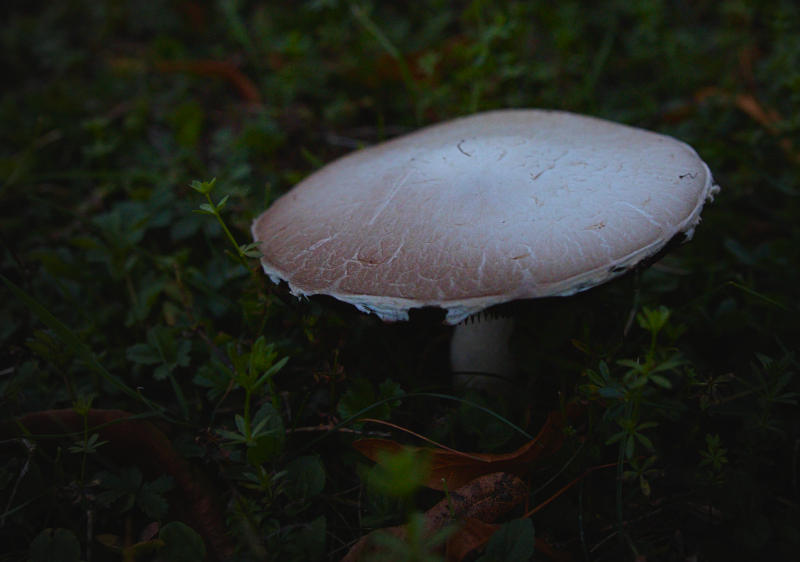
\includegraphics[width=0.25\textwidth]{images/schwammerl}
	\caption{Bild mit Textumfluss.}
	\label{fig:beispiel_umfluss}
\end{wrapfigure}

Bei sehr hohen und schmalen Bildern kann es nützlich sein, Textumfluss zu verwenden.
Dies kann in \LaTeX mit der \verb|wrapfigure|-Umgebung umgesetzt werden:

\begin{verbatim}
\begin{wrapfigure}{R}{0.3\textwidth}
	\centering
	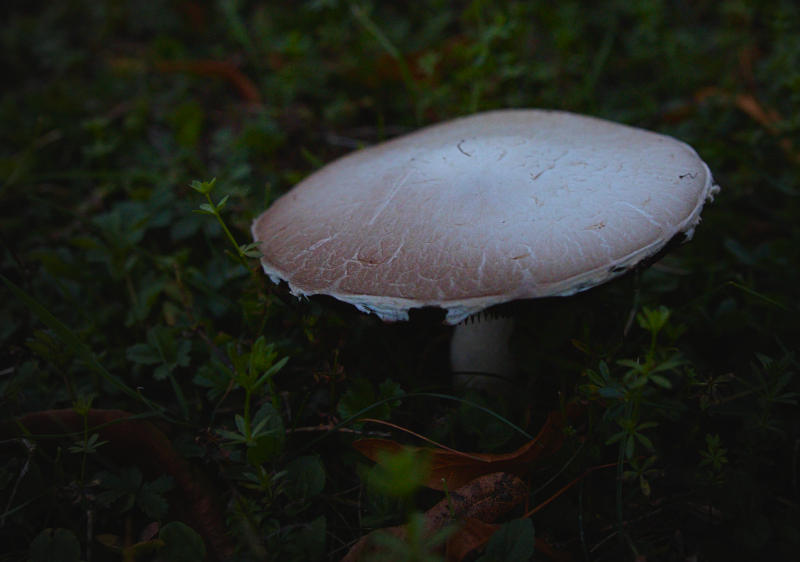
\includegraphics[width=0.25\textwidth]{images/schwammerl}
	\caption{Bild mit Textumfluss.}
	\label{fig:beispiel_umfluss}
\end{wrapfigure}
\end{verbatim}



Falls Ihre Arbeit viele Abbildungen des gleichen Formates enthält, können Sie sich folgendermaßen ein Makro als Abkürzung definieren:

\begin{verbatim}
\newcommand*{\image}[2]{
	\begin{figure}
	\centering
	\includegraphics[width=0.5\textwidth]{images/#1}
	\caption{#2}
	\label{fig:#1}
	\end{figure}
}
\end{verbatim}
Diese Definition steht in der Datei \emph{config.tex} und kann dort auch angepasst werden.

Damit erhalten Sie die Möglichkeit statt der obigen Umgebung einfach
\begin{verbatim}
\image{dateiname}{Bildbeschreibung}
\end{verbatim}
zu benutzen. Das Label erhält in diesem Fall den Namen „fig:<Dateiname>” für das Beispielbild.

\image{blume}{zweite Verwendung des Beispielbildes mit dem image-Makro. Die Datei heißt blume.jpg.}

Die Referenz \ref{fig:blume} wird dann mit \verb+\ref{fig:blume}+ erzeugt.

\minisec{Tabellen}

Tabellen in \LaTeX{} zu erstellen mag anfangs etwas umständlich erscheinen, sie bieten jedoch sehr viel gestalterische Möglichkeiten. Hier werden lediglich die einfachsten Grundlagen gezeigt.

Für die Platzierung kann, wie zu Beginn dieses Abschnittes Beschrieben die \emph{table}-Umgebung benutzt werden.

Innerhalb dieser befindet sich mit dem \emph{tabular}-Environment die eigentliche Tabelle.
Dessen Parameter bestimmen die Anzahl der Spalten, sowie die Ausrichtung der Inhalte dieser.
Über \verb|\hline| können horizontale Linien eingebaut werden.
Die Inhalte werden Zeilenweise (getrennt durch \verb|\\|) hinzugefügt und diese Zeilen werden durch das \verb|&|-Symbol in Spalten unterteilt.

Die Anpassung des Makros \verb+\arraystretch+ erhöht den Zeilenabstand. Für elegantere Lösungen betreffend Tabellen sei auf Ergänzungspakete wie tabularx \citep{latex:tabularx} oder booktabs \citep{latex:booktabs} verwiesen.

\begin{verbatim}
\begin{table}
\renewcommand{\arraystretch}{1.5}
\centering
\begin{tabular}{l|l}
\hline
\bfseries Erste Spalte& \bfseries Zweite Spalte \\
\hline
Erste Zeile & lorem \\
Zweite Zeile & ipsum \\
Dritte Zeile & dolor \\
\hline
\end{tabular}
\caption{Tabellenbeschreibung}
\label{table:label_der_tabelle}
\end{table}
\end{verbatim}

\begin{table}
	\renewcommand{\arraystretch}{1.5}
	\centering
	\begin{tabular}{l|l}
		\hline
		\bfseries Erste Spalte& \bfseries Zweite Spalte \\
		\hline
		Erste Zeile & lorem \\
		Zweite Zeile & ipsum \\
		Dritte Zeile & dolor \\
		\hline
	\end{tabular}
	\caption{Tabellenbeschreibung}
	\label{table:label_der_tabelle}
\end{table}

\minisec{Code}

Um Code einzubinden, wird das \verb|lstlisting|-Environment verwendet.
Über Parameter können Metadaten wie die Programmiersparche (wichtig für korrektes Syntax-Highlighting), die Beschreibung und das Label festgelegt werden.

\begin{verbatim}
\begin{lstlisting}[language=C++,
                   caption={Beschreibung des Codebeispiels},
                   captionpos=b,
                   label=code:code_label]
#include <stdio.h>

int main()
{
    printf("Hallo Welt!\n");
}
\end{lstlisting}
\end{verbatim}

\begin{lstlisting}[language=C++,
                   caption={Beschreibung des Codebeispiels},
                   captionpos=b,
                   label=code:code_label]
#include <stdio.h>

int main()
{
    printf("Hallo Welt!\n");
}
\end{lstlisting}

Über das \verb|verbatim|-Environment kann mehrzeiliger Code \textbf{ohne} Syntax-Highlighting, Beschreibung und Label eingebunden werden.

\verb|\begin{verbatim}|

\verb|Dieser Text ist in einer Monosaced-Schriftart geschrieben.|

\verb|Könnte z.B. für Pseudocode nützlich sein.|

\verb|\end{verbatim}|

\begin{verbatim}
Dieser Text ist in einer Monosaced-Schriftart geschrieben.
Könnte z.B. für Pseudocode nützlich sein.
\end{verbatim}

Sollen nur einzelne Wörter monospaced angezeigt werden, kann auf \verb!\verb|text|! zurückgegriffen werden: \verb|text|.

\subsubsection{Zitate und Fußnoten}

\minisec{Zitate im Text}

Zitate im Text und Einträge im Literaturverzeichnis werden aus Einträgen einer \emph{BibTeX}-Datei generiert.
Diese kann entweder selbst zusammengestellt, oder aus einem Programm zu Literatuverwaltung (z.B. Zotero, Mendeley, Citavi) exportiert werden.

Um eine Quelle zu zitieren, können folgende Befehle verwendet werden:

\bigskip

\begin{tabular}{@{}ll@{}}
\hline
\textbf{Befehl} & \textbf{Ergebnis} \\
\hline
    \verb|\cite{mustermann2013test}| & \cite{mustermann2013test} \\
    \verb|\cite[S. 15]{mustermann2013test}| & \cite[S. 15]{mustermann2013test} \\
    \verb|\citet[S. 15]{mustermann2013test}| & \citet[S. 15]{mustermann2013test} \\
\hline
\end{tabular}

\bigskip

Einträge im Literaturverzeichnis werden automatisch erstellt, wenn eine Quelle zitiert wird.

\minisec{Blockzitate}

Blockzitate werden mit dem \verb|quote|-Environment umschlossen.
Sie sollten mit einem Verweis auf die Literaturquelle beendet werden.

\begin{verbatim}
\begin{quote}
«Wenn die Wurst so[…]»
\cite[S. 4]{mustermann2013test}
\end{quote}
\end{verbatim}

\begin{quote}
«Wenn die Wurst so dick wie das Brot ist, ist es wurst wie dick das Brot ist.»
\cite[S. 4]{mustermann2013test}
\end{quote}

\minisec{Fußnoten}

Fußnoten werden über den \verb|\footnote{Inhalt der Fußnote}|-Befehl erstellt und automatisch nummeriert. Beispiel:

Informationen zum Studium der Medieninformatik an der Universität Regensburg finden Sie auf der Website des Lehrstuhls\footnote{\url{https://www.uni-regensburg.de/sprache-literatur-kultur/medieninformatik/}}.


\begin{singlespace}
\KOMAoptions{parskip=full}
% Erklärung zur Urherberschaft (urheberschaft.tex) anhängen
\addchap{Erklärung zur Urheberschaft}

Ich habe die Arbeit selbständig verfasst, keine anderen als die angegebenen Quellen und Hilfsmittel benutzt, sowie alle Zitate und Übernahmen von fremden Aussagen kenntlich gemacht. 

Die Arbeit wurde bisher keiner anderen Prüfungsbehörde vorgelegt. 

Die vorgelegten Druckexemplare und die vorgelegte digitale Version sind identisch.

\ifdefstring
{\getWorkType}{Masterarbeit}
{Von den zu § 27 Abs. 5 der Prüfungsordnung vorgesehenen Rechtsfolgen habe ich Kenntnis.}
{}

\signature


% Erklärung zur Lizenzierung der Arbeit (lizenzierung.tex) anhängen
\addchap{Erklärung zur Lizenzierung und Publikation dieser Arbeit}

\textbf{Name:} \getAuthor

\textbf{Titel der Arbeit:} \textit{\getTitle}

Hiermit gestatte ich die Verwendung der schriftlichen Ausarbeitung zeitlich unbegrenzt und nicht-exklusiv unter folgenden Bedingungen:

\begin{itemize}
    \item[\checkboxEmpty] Nur zur Bewertung dieser Arbeit
    \item[\checkboxEmpty] Nur innerhalb des Lehrstuhls im Rahmen von Forschung und Lehre
    \item[\checkboxChecked] Unter einer Creative-Commons-Lizenz mit den folgenden Einschränkungen:
    \begin{itemize}
        \item[\checkboxChecked] BY – Namensnennung des Autors
        \item[\checkboxEmpty] NC – Nichtkommerziell
        \item[\checkboxEmpty] SA – Share-Alike, d.h. alle Änderungen müssen unter die gleiche Lizenz gestellt werden.
    \end{itemize}
\end{itemize}
{\scriptsize(An Zitaten und Abbildungen aus fremden Quellen werden keine weiteren Rechte eingeräumt.)}

Außerdem gestatte ich die Verwendung des im Rahmen dieser Arbeit erstellten Quellcodes unter folgender Lizenz:

\begin{itemize}
    \item[\checkboxEmpty] Nur zur Bewertung dieser Arbeit
    \item[\checkboxEmpty] Nur innerhalb des Lehrstuhls im Rahmen von Forschung und Lehre
    \item[\checkboxEmpty] Unter der CC-0-Lizenz (= beliebige Nutzung)
    \item[\checkboxChecked] Unter der MIT-Lizenz (= Namensnennung)
    \item[\checkboxEmpty] Unter der GPLv3-Lizenz (oder neuere Versionen)
\end{itemize}

{\scriptsize(An explizit mit einer anderen Lizenz gekennzeichneten Bibliotheken und Daten werden keine weiteren Rechte eingeräumt.)}

\noindent
Ich willige ein, dass der Lehrstuhl  für Medieninformatik diese Arbeit – falls sie besonders gut ausfällt - auf dem Publikationsserver der Universität Regensburg veröffentlichen lässt.

\noindent
Ich übertrage deshalb der Universität Regensburg das Recht, die Arbeit elektronisch zu speichern und in Datennetzen öffentlich zugänglich zu machen. Ich übertrage der Universität Regensburg ferner das Recht zur Konvertierung zum Zwecke der Langzeitarchivierung unter Beachtung der Bewahrung des Inhalts (die Originalarchivierung bleibt erhalten).

\noindent
Ich erkläre außerdem, dass von mir die urheber- und lizenzrechtliche Seite (Copyright) geklärt wurde und Rechte Dritter der Publikation nicht entgegenstehen.

\begin{itemize}
    \item[\checkboxChecked] Ja, für die komplette Arbeit inklusive Anhang
    \item[\checkboxEmpty] Ja, für eine um vertrauliche Informationen gekürzte Variante (auf dem Datenträger beigefügt)
    \item[\checkboxEmpty] Nein
    \item[\checkboxEmpty] Sperrvermerk bis (Datum):
    %Sperrvermerke sind mit dem Betreuer am Lehrstuhl abzustimmen. Sperrvermerke mit einer Frist von mehr als zwei Jahren benötigen immer eine schriftliche Begründung, aus der hervorgeht, weshalb eine kürzere Sperrfrist nicht ausreichend ist.
\end{itemize}

\signature


% Stichwortverzeichnis anzeigen. Weiß nicht, warum das nicht nach dem Inhaltsverzeichnis kommt.
\printindex
\end{singlespace}

% Inhalt des Datenträgers. Gehört meiner Meinung nach zum Anhang, aber was weiß ich schon. AS
\newpage
\input{datenträger}

\end{document}
